\section{Resultados}


\subsection{Resultados Random}

A continuación observaremos una matriz en la que la única sanguijuela que se debe eliminar es la del centro. Esta se encuentra exactamente en el punto central. Adicionalmente hay otras 4 sanguijuelas en las puntas. Matar a estas no soluciona nada ya que la del centro esta aplicando una temperatura constante de 400 Cº. 

\begin{figure}[htb]
\begin{center}
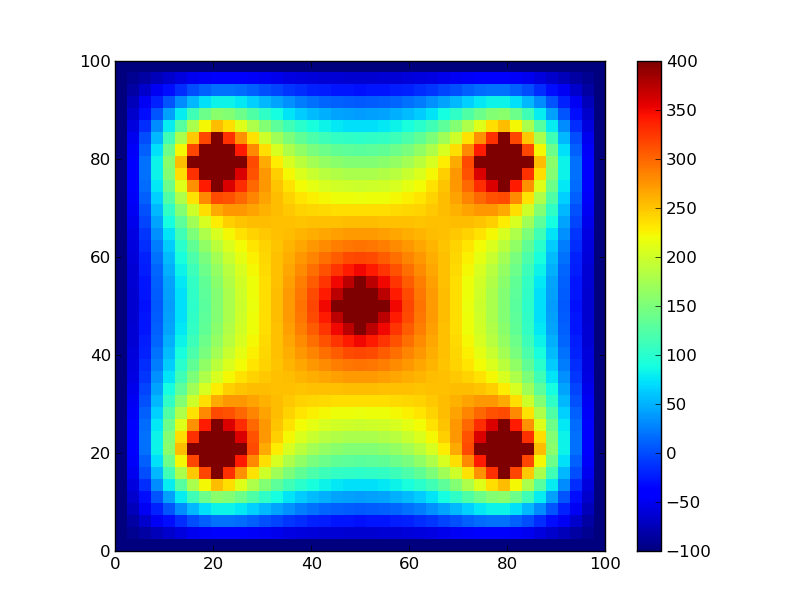
\includegraphics[scale=0.70]{imagenes/test5.png} 
\caption{Parabrisas con 5 sanguijuelas} 
\end{center}
\end{figure}


Ahora veamos que obtenemos al aplicarle distintas veces el algoritmo de solución random explicado en el desarrollo (\ref{sec:solucionRandom}).
\newpage

\begin{figure}[htb]
\begin{center}
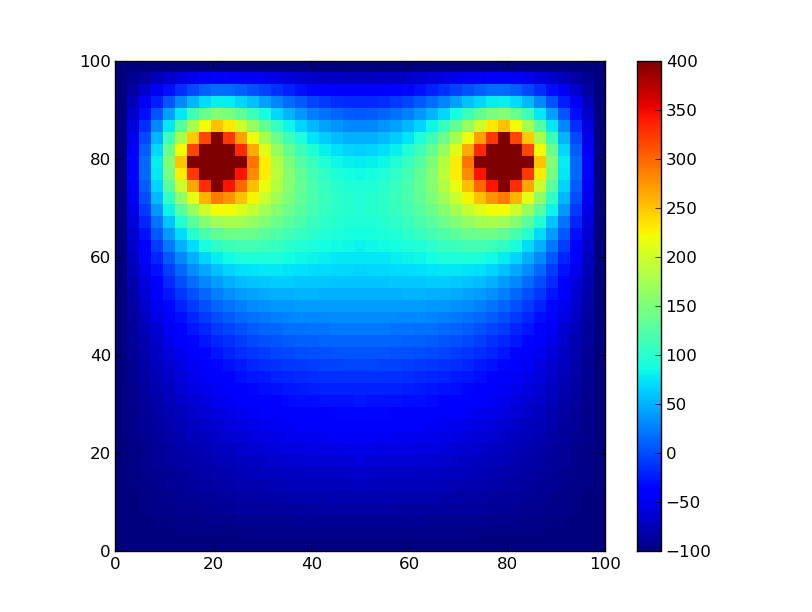
\includegraphics[scale=0.50]{imagenes/random_1.png} 
\caption{Resultado primer corrida} 
\end{center}
\end{figure}


\begin{figure}[htb]
\begin{center}
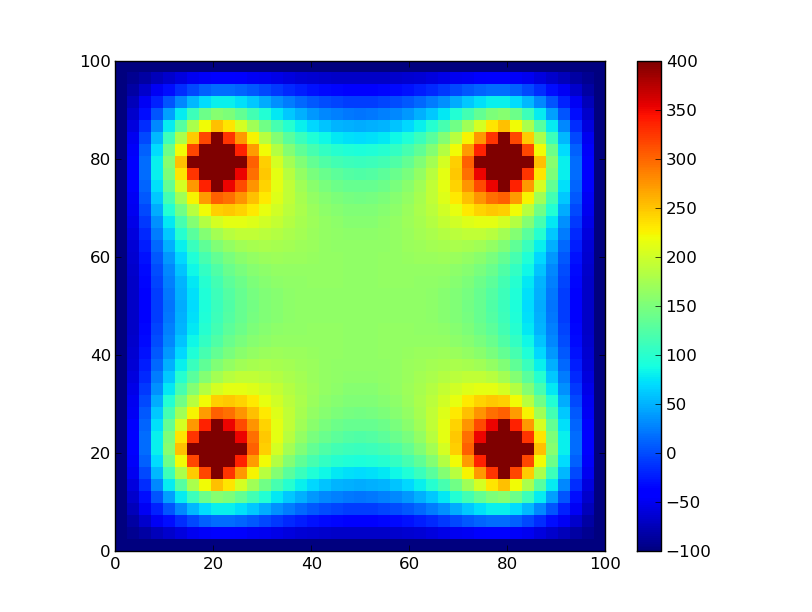
\includegraphics[scale=0.50]{imagenes/random_2.png} 
\caption{Resultado segunda corrida} 
\end{center}
\end{figure}
\newpage

\begin{figure}[htb]
\begin{center}
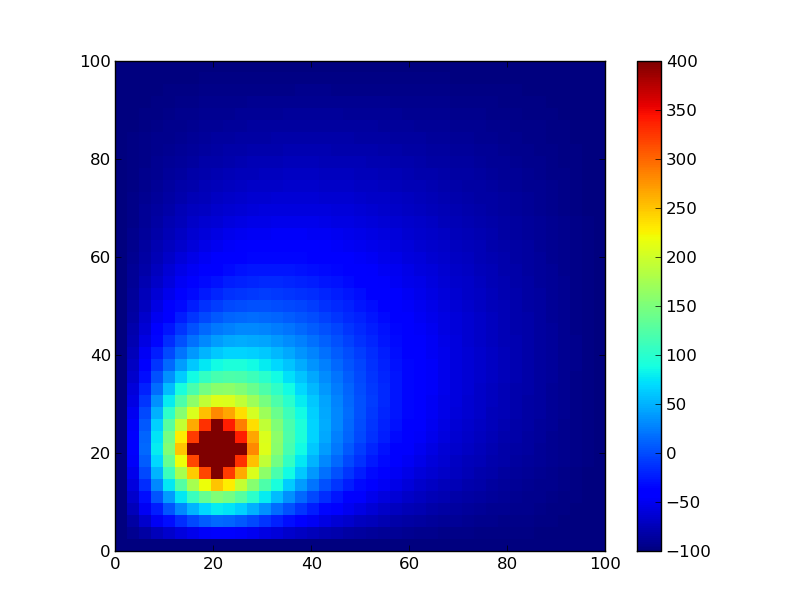
\includegraphics[scale=0.50]{imagenes/random_3.png} 
\caption{Resultado tercer corrida} 
\end{center}
\end{figure}

Como podemos observar la solución óptima (la que menos sanguijuelas elimina), es la segunda. Pero como esta solución es completamente random en la primera corrida mata 2 sanguijuelas antes de elegir la correcta y en la tercera 4. Sólo en la segunda elije en el primer intento la sanguijuela correcta.
\newpage
Veamos ahora cuanto demoró cada una de las soluciones. Es importante aclarar que acá el algoritmo utilizado para recalcular las temperaturas fue el gaussiano sin banda matriz. Para que la diferencia de tiempos sea mas clara.


\begin{figure}[htb]
\begin{center}
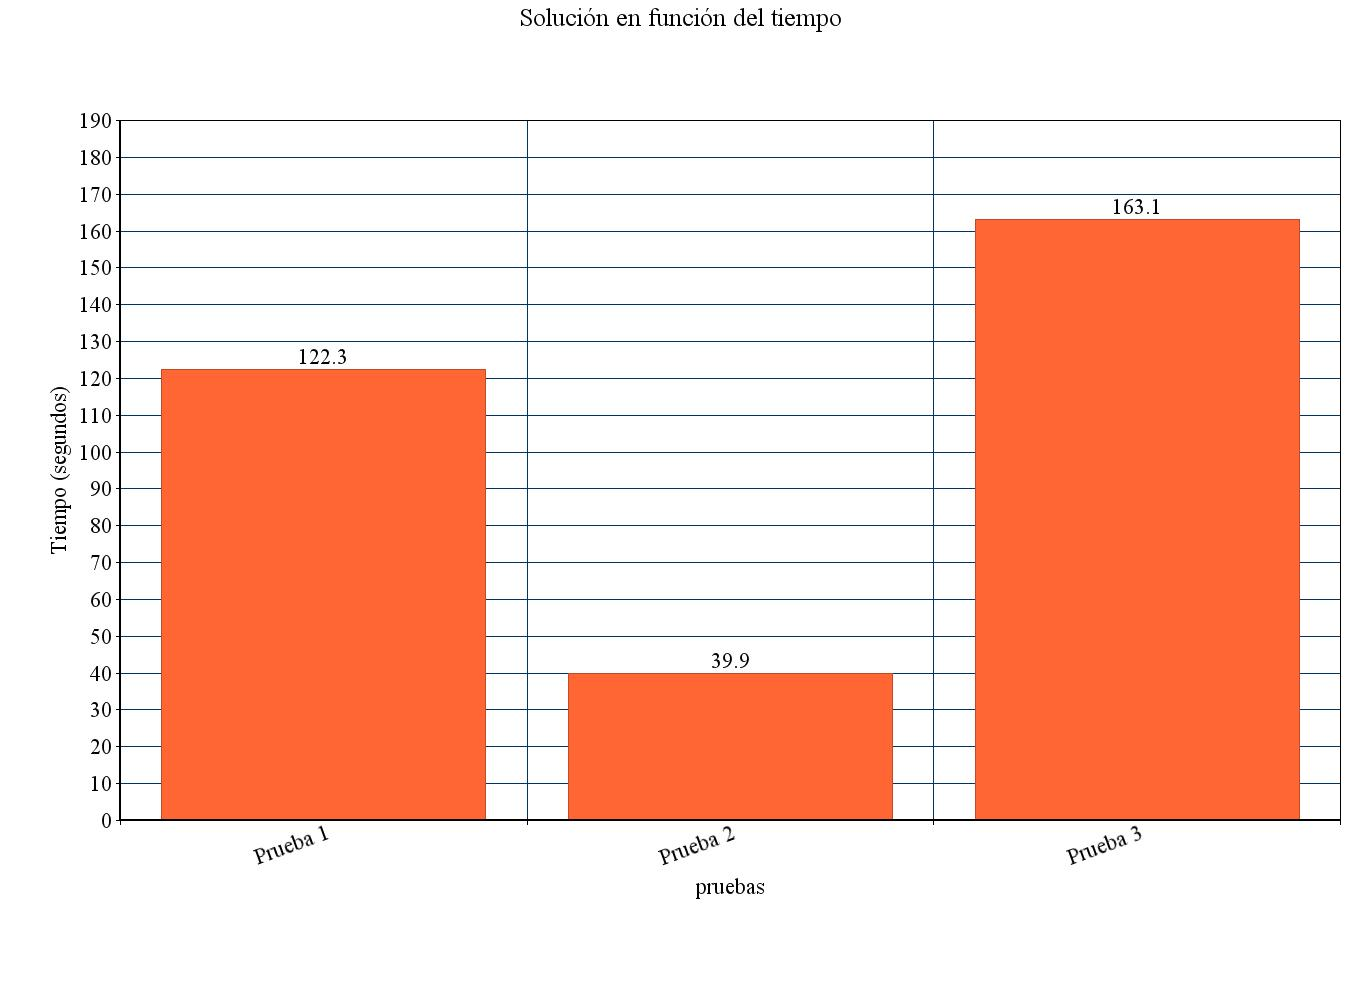
\includegraphics[scale=0.30]{imagenes/random_tiempo.jpg} 
\caption{Tiempos de corrida de cada prueba} 
\end{center}
\end{figure}

Acá podemos observar que, como era de esperarse, cuanto màs sanguijuelas elimina mas tiempo tarda, ya que debe recalcular las temperaturas.